\begin{surferPage}[Cayley-Kubik]{Die Cayley-Kubik}
  Diese Kubik (Fläche vom Grad $3$) besitzt 
    gleichzeitig vier doppelkegelförmige Singularitäten. Sie ist nach
    Arthur Cayley benannt, der viel über kubische Flächen geforscht hat.

    Es war aber Ludwig Schläfli, der als erster 1863 diese Flächen
    systematisch danach untersuchte, welche Typen von Singularitäten auftreten
    können.  
    Z.B.\ kann man in seiner Arbeit nachlesen, warum es nicht mehr als $4$
    singuläre Punkte gleichzeitig auf einer kubischen Fläche geben kann, 
    d.h.\ $\mu(3)=4$. 
    
    Auch Felix Klein untersuchte um 1900 kubische Flächen auf ihre
    möglichen Gestalten; seine Idee war es, diese Frage
    von der Cayley-Kubik ausgehend durch leichte Veränderungen zu beantworten:
    Durch Aufweiten, Auftrennen oder Zusammenführen von Doppelkegeln konnte er
    tatsächlich alle anderen Gestalten erhalten, z.B.: \newline
    \begin{center}
      \vspace{-0.2cm}
      \begin{tabular}{@{}c@{\ }c@{\ }c@{\ }c@{}}
        \begin{tabular}{@{}c@{}}
          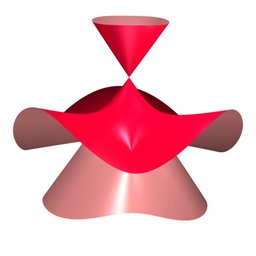
\includegraphics[width=1.35cm]{./../../common/images/cayley_cubic_0}
        \end{tabular}
        &
        \begin{tabular}{@{}c@{}}
          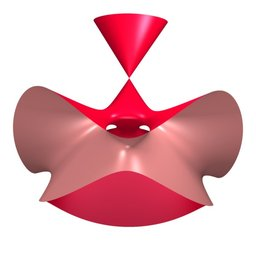
\includegraphics[width=1.35cm]{./../../common/images/cayley_cubic_1}
        \end{tabular}
        &
        \begin{tabular}{@{}c@{}}
          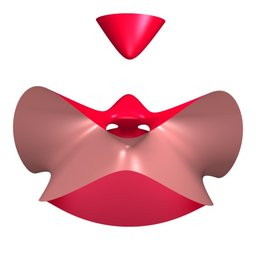
\includegraphics[width=1.35cm]{./../../common/images/cayley_cubic_2}
        \end{tabular}
        &
        \begin{tabular}{@{}c@{}}
          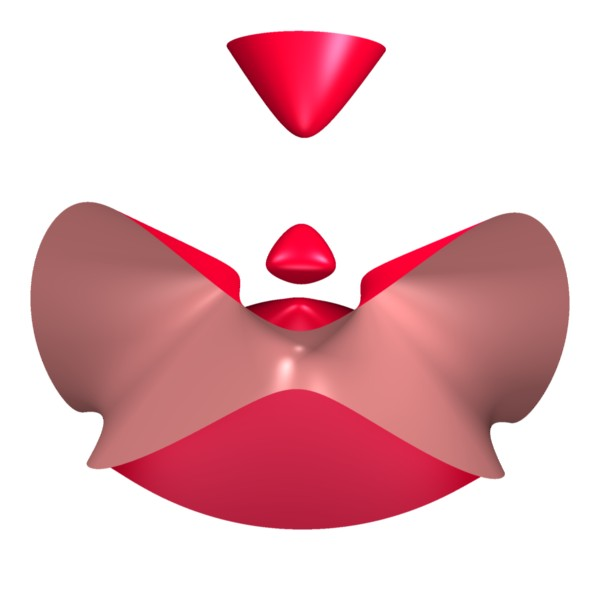
\includegraphics[width=1.35cm]{./../../common/images/cayley_cubic_3}
        \end{tabular}
      \end{tabular}
    \end{center}
\end{surferPage}
